% !TeX spellcheck = en_US
\documentclass[11pt]{article}

\usepackage[hmargin=3.1cm,vmargin=2.4cm]{geometry}
\usepackage{mathtools}
\usepackage[dvipsnames]{xcolor}
\usepackage{amssymb,dsfont,stmaryrd}
\usepackage{algorithm2e}
\usepackage{hyperref,cleveref}
\usepackage{graphicx}
\usepackage{booktabs}
\usepackage{subcaption}
\usepackage{enumitem}
\usepackage[noindentafter]{titlesec}
\usepackage{tikz}

\usetikzlibrary{bayesnet,arrows,backgrounds}


\setlist{itemsep=0pt}

\hypersetup{
	urlcolor=NavyBlue
}

%%% Math macros %%%

\newcommand\RR{\mathbb{R}}
\newcommand\CC{\mathbb{C}}
\newcommand\ZZ{\mathbb{Z}}
\newcommand\NN{\mathbb{N}}
\newcommand\TT{\mathbb{T}}
\newcommand\PP{\mathbb{P}}
\newcommand\EE{\mathbb{E}}
\DeclarePairedDelimiter{\intinterv}{\llbracket}{\rrbracket}

\renewcommand{\epsilon}{\varepsilon}

\newcommand{\suchthat}{\mathrm{s.t.}}

\DeclareMathOperator*{\argmin}{\mathrm{argmin}}
\DeclareMathOperator*{\argmax}{\mathrm{argmax}}
\DeclareMathOperator{\diag}{\mathrm{diag}}
\DeclareMathOperator{\sgn}{\mathrm{sgn}}
\DeclareMathOperator{\trace}{\mathrm{Tr}}

\newcommand{\calM}{\mathcal{M}}
\newcommand{\calP}{\mathcal{P}}
\newcommand{\calN}{\mathcal{N}}
\newcommand{\calX}{\mathcal{X}}
\newcommand{\calL}{\mathcal{L}}
\newcommand{\calC}{\mathcal{C}}
\newcommand{\calD}{\mathcal{D}}

\newcommand{\bmmu}{\boldsymbol{\mu}}
\newcommand{\bmpsi}{\boldsymbol{\psi}}
\newcommand{\bmphi}{\boldsymbol{\phi}}

\newcommand{\bmX}{\boldsymbol{X}}

\colorlet{darkblue}{NavyBlue!80!black}
\newcommand{\bluefont}{\color{darkblue}}


%%% Section titling setup %%%

\titleformat*{\section}{\LARGE\bfseries\sffamily}
\titleformat*{\subsection}{\Large\bfseries\sffamily}

\titleformat{\paragraph}[hang]{\sffamily\bfseries}{}{}{}[]


%%% Document title %%%

\title{
	MVA -- Probabilistic Graphical Models\\
	{\color{NavyBlue}\sffamily Homework 3: Gibbs Sampling and VB}
}

\author{
	Wilson \textsc{Jallet}\thanks{\url{wilson.jallet@polytechnique.org}}}


\begin{document}

\maketitle


\paragraph{Question 1}
This operation puts all the data on the same scale -- this is especially useful because the prior on $\beta$ assigns the same variance in each direction.


\paragraph{Question 2}
If we supposed that $\epsilon_i$ had a variance of $\sigma^2$, we could write $\epsilon_i = \sigma \epsilon'_i$ where $\epsilon'_i \sim \calN(0,1)$, and we'd have
\[
	y_i = \sgn(\beta^T x_i + \epsilon_i) =
	\sgn({\beta'}^T x_i + \epsilon'_i)
\]
where $\beta' = \beta/\sigma$.


\paragraph{Question 3}
We define the following graphical model:
\begin{itemize}
	\item observed features $x_i \in \RR^p$, $i\in\{1,\ldots,n\}$
	\item random variable $\beta\sim \calN(0, \tau I_p)$
	\item latent variables $z_i = \beta^Tx_i + \epsilon_i$, $\epsilon_i \sim \calN(0,1)$
	\item observed labels $y_i = \sgn(z_i) \in \{-1,1\}$
\end{itemize}
It has the following representation:
\begin{figure}[h]
	\centering
	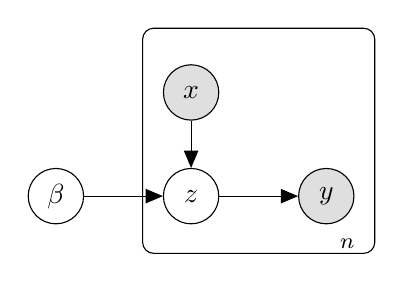
\begin{tikzpicture}
	\node[obs] (y) {$y$};%
	\node[latent,left=of y] (z) {$z$}; %
	\node[latent,left=of z] (beta) {$\beta$}; %
	\node[obs,above=of z,yshift=-4mm] (x) {$x$};
	% plate
	\plate [inner sep=.25cm,yshift=.2cm] {plate1} {(x)(y)(z)} {$n$}; %
	% edges
	
	\edge {x} {z};
	\edge {z} {y};
	\edge {beta} {z};
	
	\end{tikzpicture}
\end{figure}

To perform inference on the model, we need the posterior distribution of $\beta, z$ given the data $X,y$.

Our first approach is to use Gibbs sampling. To use it, we need to derive the conditional posteriors of the variables.
Evidently,
\begin{align*}
	p(y_i|\beta)
	= \Phi(y_i\beta^Tx_i)  \\
	p(z_i | \beta)  \sim \calN(\beta^T x_i, 1)  \\
	p(y_i,z_i|\beta) = \mathds{1}_{\{y_iz_i > 0\}}
\end{align*}
By Bayes' theorem we have the posteriors
\begin{align*}
	p(\beta|z) \propto p(\beta)p(z|\beta)
	&\propto \exp\left(
		-\frac1{2\tau}\|\beta\|^2
		-\frac{1}{2}\sum_{i=1}^{n}(z_i - \beta^T x_i)^2
	\right)  \\
	&= \exp\left(
		-\frac1{2\tau}\|\beta\|^2
		-\frac{1}{2}\|z - X\beta\|^2
	\right)
\end{align*}
and
\begin{align*}
	p(z|\beta,y) \propto p(z|\beta)p(y,z|\beta)
	&\propto \exp\left(
	-\frac{1}{2}\|z - X\beta\|^2
	\right) \prod_{i=1}^{n} \mathds{1}_{\{y_iz_i > 0\}}
\end{align*}
where $X = (x_1|\ldots|x_n)^T \in \RR^{n \times p}$ is the design matrix. By identification $\beta|z \sim \calN(\mu_p, \Sigma_p)$ where
\begin{equation}\label{eq:BetaPostZ}
\bluefont
	\Sigma_p^{-1} = \frac{1}{\tau}I_p + X^TX,
	\quad
	\mu_p = \Sigma_p X^Tz
\end{equation}
and $z|\beta,y \sim \mathrm{T}\calN(X\beta, I_n; \calP_y)$ where $\mathrm{T}\calN(\cdot; \calP_y)$ is the truncated Gaussian with support in the polytope $\calP_y = \{z\in\RR^n : z_i y_i > 0,\ i=1,\ldots,n\}$.

With all this in place, we use Gibbs sampling to sample from the posterior distribution of $\beta,z$ given the data $(X,y)$.
For inference and testing, we \textbf{\boldmath split the dataset up as $2/3$rds for training and $1/3$rd for testing}. \Cref{fig:GibbsMarginals} shows approximate posterior marginals for $\beta,z | X,y$ in the form of histograms made from samples.

The testing accuracy (predicting using MAP) is of about $\approx 75\%$, using 4000 samples of $\beta|X_\mathrm{train},y_\mathrm{train}$.

\begin{figure}
	\centering
	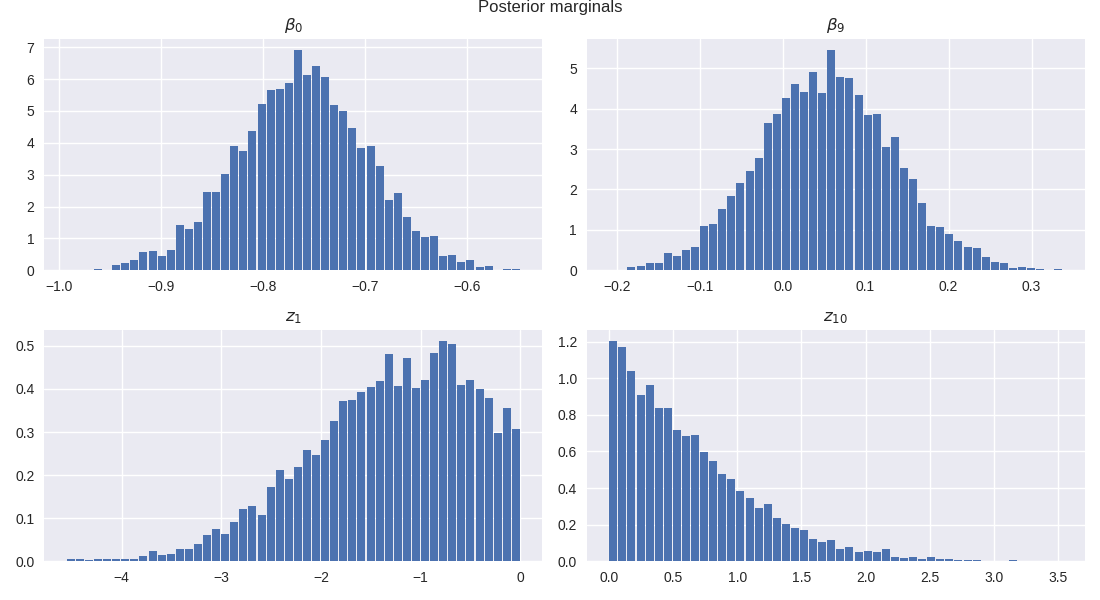
\includegraphics[width=.96\linewidth]{images/posterior_distribution_gibbs.png}
	\caption{Some approximate posterior marginals for $\beta$ and $z$ given the data $X, y$.}\label{fig:GibbsMarginals}
\end{figure}


\paragraph{Question 4}
We assume the factorization for the variational distribution $q$:
\begin{equation}
	q(\beta, z) = q_1(\beta)q_2(z)
\end{equation}

\textbf{Joint probability.} The log-joint probability is written as
\begin{equation}
\begin{aligned}
	\ln p(\beta, z, y)
	&= \ln p(y | z) + \ln p(z|\beta) + \ln p(\beta)  \\
	&= \ln p(y|z) - \frac{1}{2}\|z-X\beta\|^2 - \frac{1}{2\tau} \|\beta\|^2 + \mathrm{cst}
\end{aligned}
\end{equation}

\textbf{Derivation of \boldmath$q_1$.} The optimal form of the factor is
\begin{equation}
\begin{aligned}
	\ln q_1^*(\beta) &= \EE_{z}\left[
		\ln p(y|z) - \frac{1}{2}\|z-X\beta\|^2 - \frac{1}{2\tau} \|\beta\|^2
		\middle| \beta
	\right] + C_1  \\
	&= \EE_z [\ln p(y|z) | \beta]
	- \frac{1}{2} \underbrace{\EE_z\left[\|z-X\beta\|^2 \middle| \beta\right]}_{=\EE_{\epsilon\sim\calN(0,1)}[\|\epsilon\|^2] = 1}
	- \frac{1}{2\tau}\|\beta\|^2
	+ C_2
\end{aligned}
\end{equation}
Since
\[
	\ln p(y|z) = \sum_{i=1}^n \mathds{1}_{y_i=1}\ln(\mathds{1}_{z_i>0}) + \mathds{1}_{y_i=-1}\ln(\mathds{1}_{z_i\leq 0})
\]
the first term is
\[
	\EE_z[\ln p(y|z) | \beta] =
\]
The end result is
\begin{equation}
\bluefont
	\ln q^*_1(\beta) = -\frac{1}{2\tau}\|\beta\|^2 + C_3
\end{equation}
so $\boxed{q^*_1 = \calN(0, \tau I_p).}$


\textbf{Derivation of \boldmath$q_2$.} The optimal form of the factor is
\begin{equation}
	\ln q_2^*(z) = \EE_{\beta}\left[
	\ln p(y|z) - \frac{1}{2}\|z-X\beta\|^2 - \frac{1}{2\tau} \|\beta\|^2
	\middle| z
	\right] + C_4
\end{equation}
It holds that
\[
\begin{aligned}
	\EE_\beta \left[
		\|\beta\|^2 + \|z-X\beta\|^2 \middle| z
	\right]
	&=
	\EE_\beta\left[
	(\beta - \mu_p)\Sigma_p^{-1}(\beta - \mu_p) + C(z)
	\middle| z
	\right] \\
	&= \underbrace{\EE_{u\sim \calN(\mu_p,\Sigma_p)}\left[
	(u - \mu_p)^T \Sigma_p^{-1}(u - \mu_p)
	\middle| z
	\right]}_{=1} + C(z)
\end{aligned}
\]
where $(\mu_p,\Sigma_p)$ come from \cref{eq:BetaPostZ}, and $C(z)$ is the difference between the terms under the expectations on the first line. Evaluating the expression with $\beta = 0$ leads to
\[
	C(z) = \|z\|^2 - \mu_p(z)^T \Sigma_p^{-1}\mu_p(z)
	= \|z\|^2 - z^T X\Sigma_p X^T z =
	z^T(I_p - X\Sigma_pX^T)z
\]
The expectation $\EE_y[\ln p(y|z) \mid z]$ is still $0$.
This leads to
\begin{equation}
\begin{aligned}
	\ln q_2^*(z) &=
	-\frac{1}{2} z^T (I_p - X\Sigma_p X^T)z + C_5
\end{aligned}
\end{equation}
i.e. $\boxed{q_2^* = \calN(0, I_p - X\Sigma_pX^T).}$

\end{document}
